\documentclass{article}
\usepackage{color}
\usepackage[UTF8]{ctex}
\usepackage{graphicx}
\usepackage{float}

\begin{document}
    \title{第一次实验}
    \author{汤琦 \\ 23020007110\\ https://github.com/wlmrh/System-development-tool-basics}
    \date{\today}
    \maketitle

    \pagenumbering{arabic}
    \tableofcontents
    \newpage

    \setlength{\parindent}{0pt}
    \setcounter{page}{1}
    \sloppy

    \section{Latex简单使用}
        \subsection{形成基础结构}
        使Latex支持中文字体: \verb|\usepackage[UTF8]{ctex}|(使用CTex宏包)\\
        全局去除Latex默认的段首空格: \verb|\setlength{\parindent}{0pt}|(即将段首空
        格设置为0pt)\\
        添加空行:\verb|\hspace*{\fill}\\|(即用空格填充一行再换行,以此来达到视觉上的
        空行效果)\\
        遇到报错:\verb|Underfull \hbox (badness 10000)|, 报错原因为Latex无法很好
        的处理\verb|\verb|指令, 应加入\verb|\sloppy|启用宽松排版, 使其自动处理长行。

        \subsection{制作目录}
            \subsubsection{问题一}
            在创建目录时, 发现起始页对应的序号为1\\
            \hspace*{\fill} \\
            解决方法:\\
            在正文开始前,使用命令\verb|\setcounter{page}{1}|,将开始页的标号设置为1。

        \subsection{公式输入}
            与markdown类似
            \begin{equation}
            e=mc^2
            \end{equation}

            \begin{equation}
            \pi = \frac c d
            \end{equation}

            \begin{equation}
            \frac{d}{dx}e^x=e^x
            \end{equation}

            \begin{equation}
            \frac{d}{dx} \int _0 ^\infty {f(s)ds} = f(s)
            \end{equation}

            \begin{equation}
            f(x) = \mathop{\Sigma} _i 0^{\infty} \frac{f^{(i)}(0)}{i!}x^i
            \end{equation}

            \begin{equation}
            x = \sqrt{\frac{x_i}{z}y}
            \end{equation}

        \subsection {字体样式}
            使用诸如 \verb|\textit{words in italics}| 等指令, 可以改变字体。
            \hspace*{\fill} \\
            导入\verb|\usepackage{color}|导入包后可以通过\verb|\color{颜色名称}|来改变字体颜色, 
            该项默认作用于全局,可以使用\verb|{}|来缩小该指令的作用域。\\
            \hspace*{\fill} \\
            使用\verb|\tiny, \scriptsize, \large|等指令可以调整字体大小, 如: \\
            \verb|{\color{cyan}\Large text}|指令的执行效果如下, 其颜色为cyan, 大小为large\\
            {\color{cyan}\Large text}\\
            \hspace*{\fill} \\
            使用\verb|\colorbox{magenta}{\color{cyan}\Huge Hello}|的执行效果如下, 其背景
            为magenta, 字体颜色为cyan, 字体大小为huge\\
            \colorbox{magenta}{\color{cyan}\Huge Hello}

        \subsection{表格制作}
            先确定列数, 列之间是否有竖线,每一列的对齐方式: 左对齐(l), 右对齐(r), 向中对齐(c), 
            将这些参数写到begin指令的右边, 然后使用指令画出横线, 下面是oiwiki中表格部分
            对应的两道练习题。\\
            \begin{tabular}{|c|c|c|}
            \hline
            Item   & Quantity & Price(\$) \\
            \hline
            Nails  & 500      & 0.34\\
            Bricks & 240      & 11.50\\
            \hline
            \end{tabular}

            \hspace*{\fill} \\
            \begin{tabular}{c|ccc}
            & Year & & \\
            \cline{2-4}
            City & 2006 & 2007 & 2008\\
            \hline
            London & 45789 & 46551 & 51298\\
            Berlin & 34549 & 32543 & 29870\\
            Paris  & 49835 & 51009 & 51970\\

            \end{tabular}
        \newpage
    
    \sloppy
    \section{Git简单使用}
    阅读了Pro Git中的部分内容,下面是对课程配套课后练习的作答。
        \subsection{Exercise2}
            克隆本课程网站的仓库\\
            在连接中查询到本课程的仓库地址,在目标文件夹中右键点击在终端中打开, 输入指令
            \begin{verbatim}
            git clone https://github.com/missing-semester-cn/
            missing-semester-cn.github.io.git
            \end{verbatim}
                
            \begin{enumerate} 
                \item 将版本历史可视化并进行探索\\
                通过命令\verb|git log|来显示历史日志,通过参数\verb|--graph|来获取可视化视图
                \begin{figure}[H]
                    \centering
                    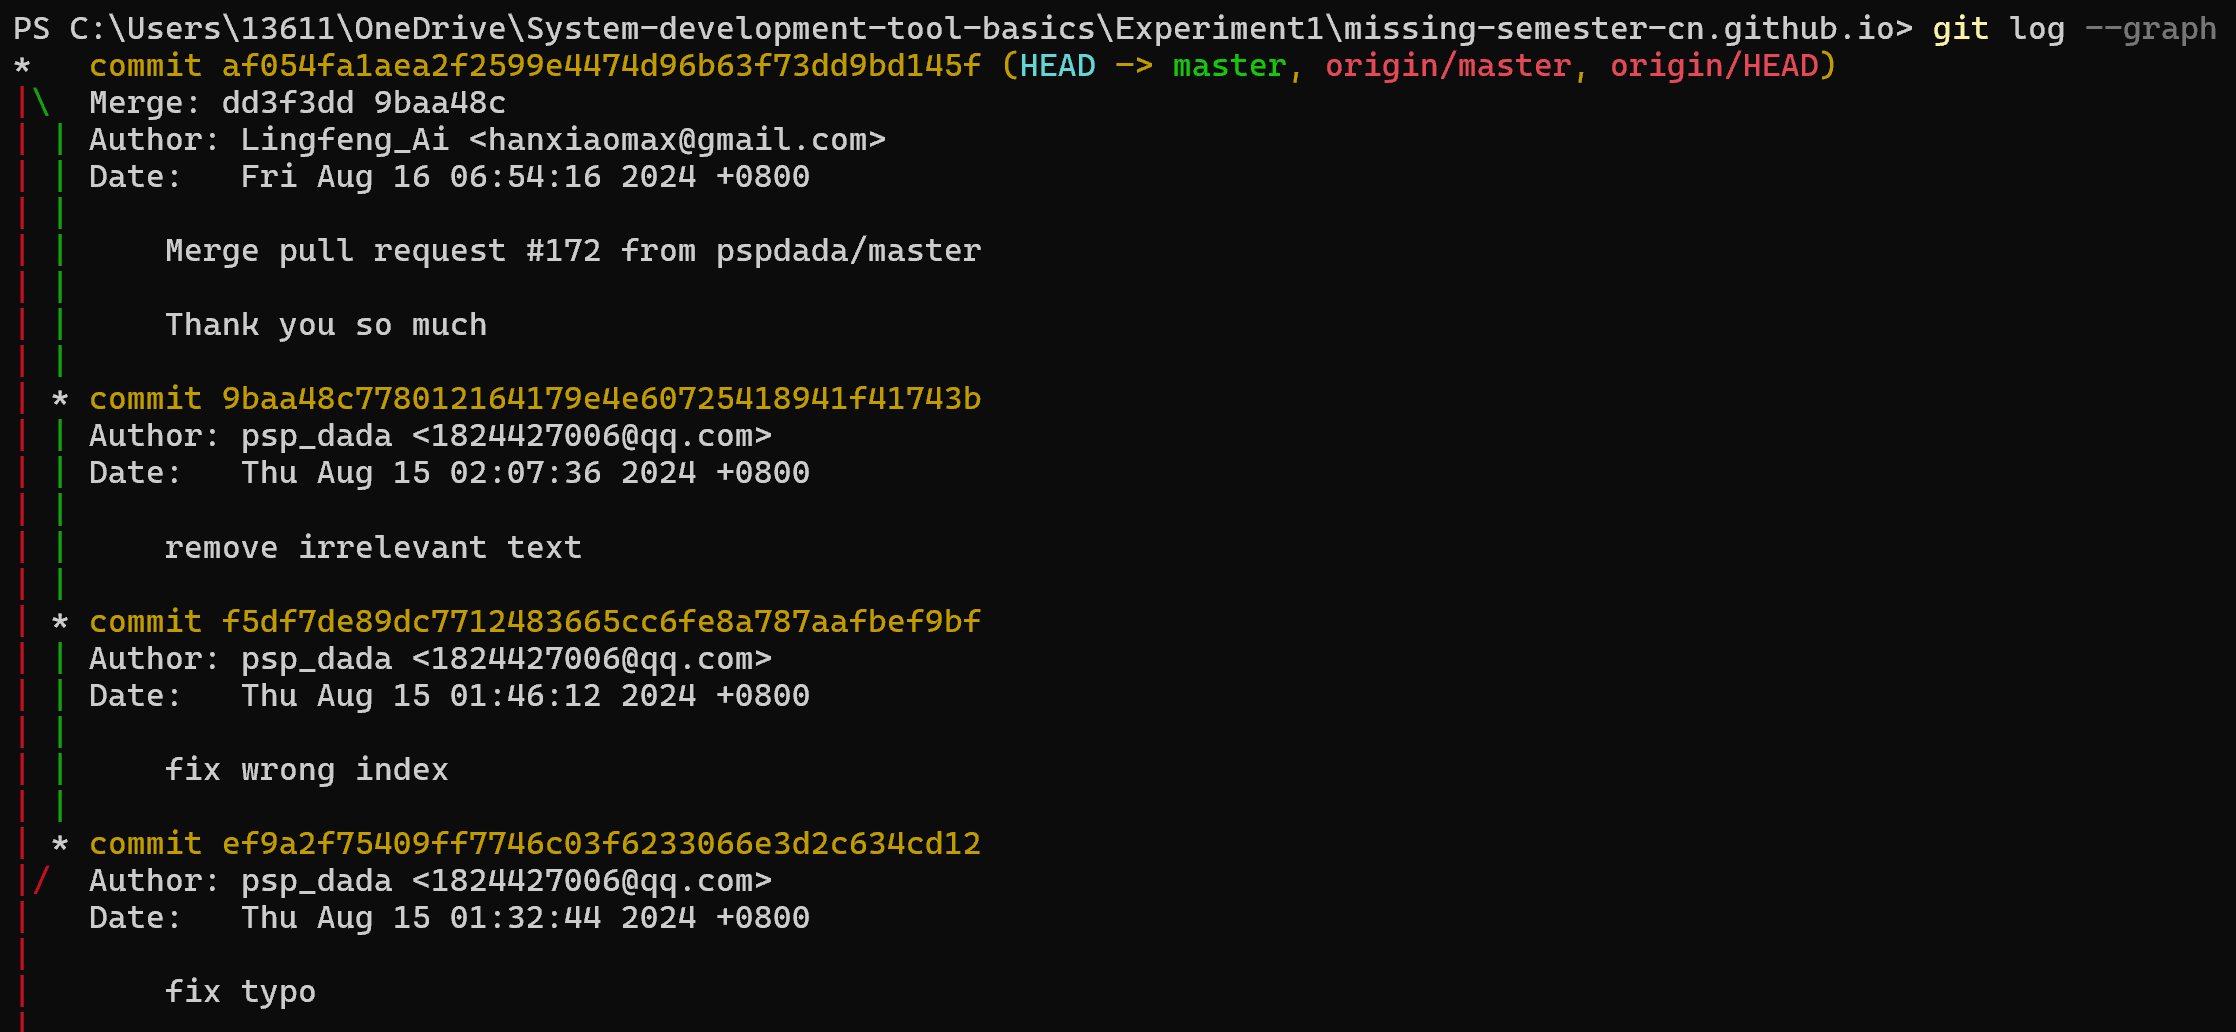
\includegraphics[scale=0.4]{1.png}
                    \caption{版本历史可视化}
                \end{figure}
                \item 是谁最后修改了 \verb|README.md| 文件?(提示:使用 \verb|git log| 命令并添加合适的参数)\\
                使用指令\verb|git log -1 (--) README.md|,其中-1表示只显示最后一次的commit, 
                \verb|--|告诉Git后面的是文件路径而不是分支名, 但在本题中不存在冲突, 可以省略, 
                \verb|README.md|则将搜索范围限制到对\verb|README.md|的修改。
                \begin{figure}[H]
                    \centering
                    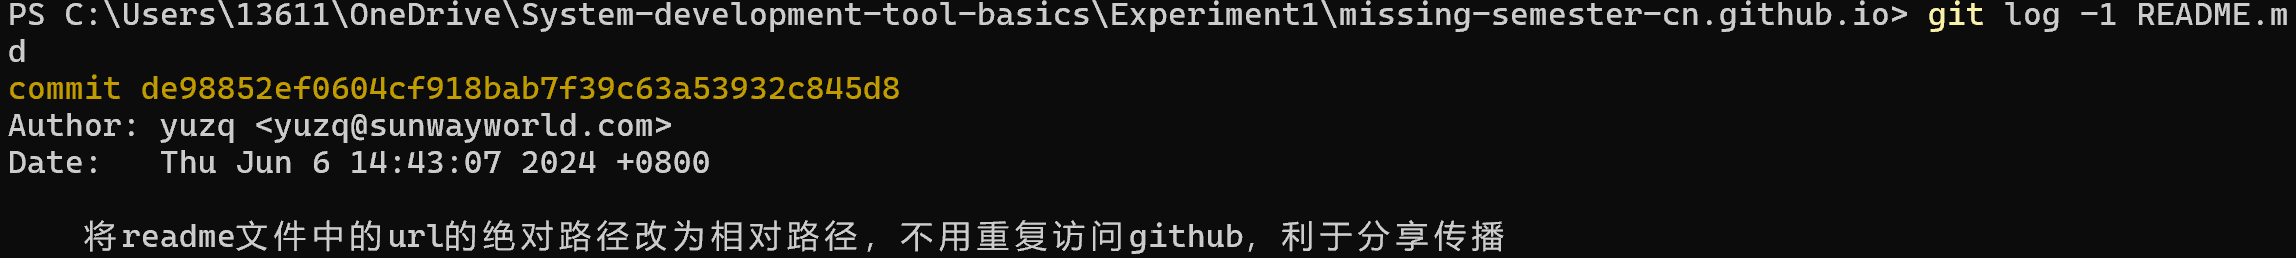
\includegraphics[scale=0.35]{2.png}
                    \caption{README.md最后一次修改}
                \end{figure}
                \item 最后一次修改 \verb|_config.yml| 文件中 collections: 行时的提交信息是什么?(提示:使用 \verb|git blame| 和 \verb|git show|)\\
                先运行\verb |git blame _config.yml|获取对 \verb|_config.yml| 进行的所有修改, 
                通过管道运算符, 将其输出作为 grep 指令的输入, 筛选出对 collections 行的提交信息。
                \begin{figure}[H]
                    \centering
                    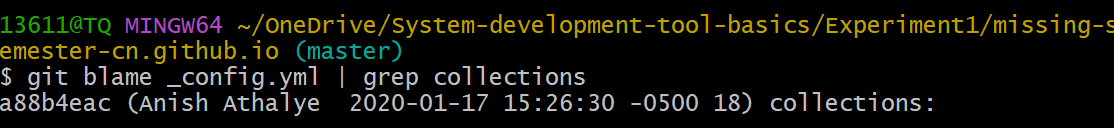
\includegraphics[scale=0.7]{3.png}
                    \caption{最后一次行修改}
                \end{figure}
            \end{enumerate}
        \subsection{Exercise4}
        从 \verb|GitHub| 上克隆某个仓库,修改一些文件。当您使用 \verb|git stash| 会发生什么?当您执行
        \verb|git log --all --oneline| 时会显示什么?通过 \verb|git stash pop| 命令来撤销
        \verb|git stash| 操作,什么时候会用到这一技巧?\\
        运行\verb|git stash|命令后, 使用\verb|git status|命令, 发现之前做的修改消失了。
        \begin{figure}[H]
            \centering
            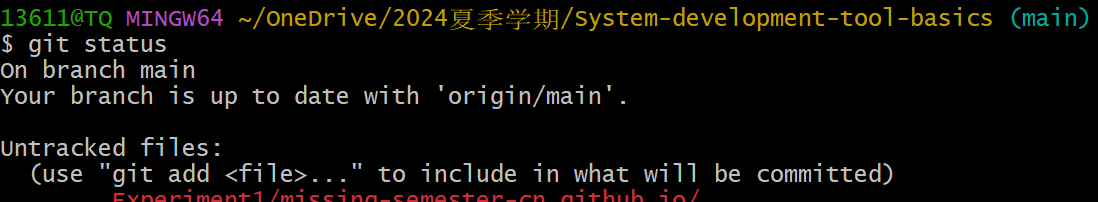
\includegraphics[scale=0.7]{4.png}
            \caption{运行后的结果}
        \end{figure}
        执行\verb|git log --all --oneline|后, 运行结果如下:
        \begin{figure}[H]
            \centering
            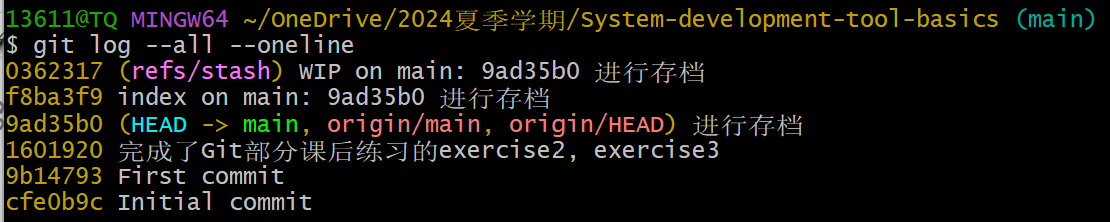
\includegraphics[scale=0.7]{5.png}
        \end{figure}
        看到之前做的修改被保存为 main 分支上的WIP(work in progress), 只是从文件夹中被移除。
        在运行指令\verb|git stash pop|指令后发现之前修改的 \verb|README.md| 
        又回到了Changes not staged for commit 中
        \begin{figure}[H]
            \centering
            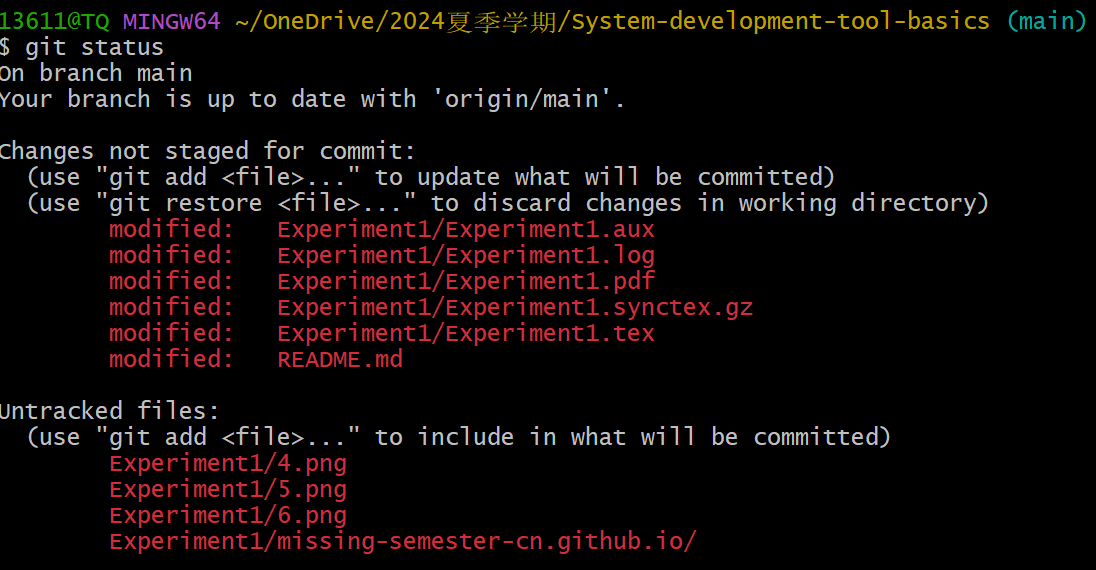
\includegraphics[scale=0.8]{6.png}
        \end{figure}
        推测 \verb|git stash|是为了在本地暂存已进行的修改而不进行提交, 
        以进行其他活动。使用场景可能是在进行功能开发时, 发现有其他bug需要维修
        这时可以在本地暂存已进行的开发, 而不用进行一次无用的提交来达到缓存的目的。
        \subsection{Exercise5}
        与其他的命令行工具一, Git 也提供了一个名为 ~/.gitconfig 配置文件 
        (或 dotfile)。请在 ~/.gitconfig 中创建一个别名,使您在运行
         git graph 时,您可以得到 git log --all --graph --decorate --oneline 
         的输出结果。\\
         只需在\verb|.gitconfig|文件中添加
         \begin{verbatim}
            [alias]
            graph = log --all --graph --decorate --oneline
        \end{verbatim}
        结果如下:
        \begin{figure}[H]
            \centering
            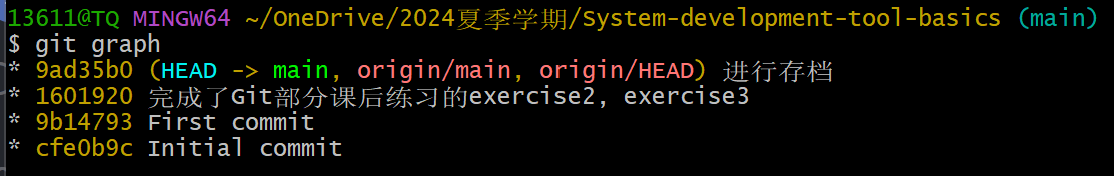
\includegraphics[scale=0.8]{7.png}
        \end{figure}
\end{document}
